\subsection{Excercise UMEGeneralConcepts}
\label{sec:ume_general_concepts}
This task provides a general overview of the general concepts of the Unified Microservice Engineering (UME) approach.
The following sections will explain the general architectural style, the domain modeling process, and the modeling of the architecture.

\subsubsection*{Architectural Style}
The Unified Microservice Engineering approach aligns with the microservices architectural style.
This involves breaking down an application into smaller, independent services that can be developed, deployed, and scaled separately.
The services communicate with each other through APIs and are usually organized around business capabilities.
These services aim to enhance flexibility, scalability, and maintainability.

Predecessors of the microservices architectural style are the service-oriented architecture (SOA) and the distributed systems architectural style which will be further explained in the following.

\paragraph*{Service Oriented Architecture}
SOA shares some similarities with the microservices architectural style.
The focus is on organizing services around business capabilities and developing them independently.
This aims to achieve reusability and interoperability.

Yet, microservices tend to be generally smaller, more fine-grained, decoupled and are usually lightweight.

\paragraph*{Distributed Systems}
Distributed systems represent a collection of independent computers, appearing to the users of the system as a single coherent system.
These systems handle tasks across a network, each node having its local memory and set of responsibilities.

Microservices share a similar idea: Splitting an application into smaller, more independent services communicating with each other.
Each microservice manages its functionalities and data to provide the overall functionality of the application.

\subsubsection*{Domain Modelling}
A domain model describes selected aspects of a domain in a conceptual model, yet the model should not separate the concept from the implementation.
This model can be used to better understand the domain and to communicate with stakeholders.

The domain model is located in the domain logic layer of the layered architecture.
Therefore each microservice implements its domain model.

Using a layered software architecture, the business logic layer is separated into application logic and domain logic.
The application logic layer contains the application-specific logic while the domain logic layer contains the domain-specific logic.
This domain-specific logic is derived from the domain model, enabling the domain knowledge to be encapsulated in the domain logic layer.
The application logic layer is derived from the analysis of the application requirements, for instance, use cases.

Therefore the domain logic layer is the part of the software architecture that is shaped the most by domain modeling.

\subsubsection*{Modelling of the Architecture}
To model the architecture of a microservice-based application, UME uses the Unified Modeling Language (UML).
To create the according diagrams, the UMLet tool \cite{UML-WEB} is used.

Two general views are distinguished: The \textbf{Application Software View} and the \textbf{Application System View}.
Both views have an artifact as their main result.
The application software view takes a logical approach and focuses on the software architecture.
Its artifact is the \textbf{Component Diagram}.
The application system view takes a physical approach and focuses on the system architecture.
Its artifact is the \textbf{Deployment Diagram}.

Both diagrams can be combined by using the \textbf{SystemPlusSoftware Diagram}.
It combines both the Component and the Deployment Diagram by putting the logical components into the physical nodes.

\subsection{Excercise APIStyles}
\label{sec:api_styles}
This task focuses on the different API styles used in the UME approach.
The following sections will explain ReST and gRPC and their properties, focusing on their usage, execution, similarities and differences.

\subsubsection*{ReST and gRPC}
\label{subsec:rest_and_grpc}
Representational state Transfer (ReST) and Remote Procedure Call (gRPC) are two different frameworks and collections of best practices and technologies for building APIs.

The main conceptual difference is the focus and orientation of both concepts:
ReST is resource-oriented.
Each resource has a unique identifier (URI) and can be accessed using the standardized HTTP methods.
Therefore, there is only a small set of well-defined methods for manipulating the resources.
gRPC is procedure, method, or function-oriented.
It is based on the idea of implementing a service, offering remotely callable methods.
These methods can be called by a client with their parameters and return values.

Both concepts have their legitimate use cases, yet it is important to choose the right one for the given use case.

\subsubsection*{ReST Properties}
ReST provides a concept of how microservices' APIs should be designed.
Its main properties are explained in the following.

\paragraph*{Addressable Ressources:}
As mentioned before, ReST is resource-oriented meaning that each resource has a unique identifier, a URL, and can be accessed using the standardized HTTP methods.
Therefore only a small set of functions is needed to manipulate the resources, offering a uniform interface.

\paragraph*{Stateless Communication:}
ReST is stateless meaning that each request is independent of the previous one.
The server, therefore, does not need to store any information about the client.
The client must transfer all the information in the request that is needed to process it to the server.
This leads to a loss of performance.
Yet, this is a tradeoff for an increase in scalability and robustness.

\paragraph*{Representation Orientation:}
This principle strongly relates to resources.
These resources have to be represented.
This happens in a standardized format, for instance, JSON or XML.
The client can choose the format that suits him best.
MIME, the Multipurpose Internet Mail Extensions standard, defines the different formats used in Internet protocols.

\begin{figure}
    \centering
    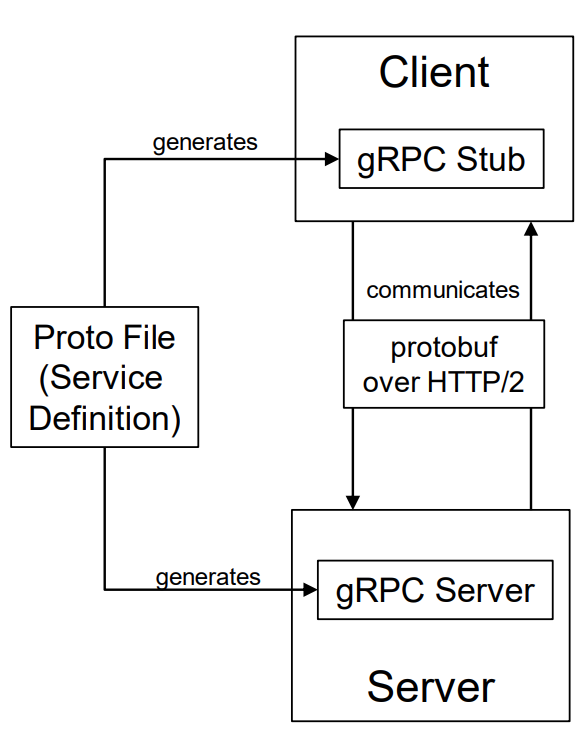
\includegraphics[width=0.4\textwidth]{figures/microservices/microservices_grpcMainComponents.png}
    \caption{Main Components of the gRPC Architecture}
    \label{fig:grpc_main_components}
\end{figure}

\subsubsection*{gRPC Components}
% Name and describe the main components of the gRPC architecture.
gRPC is an open-source remote procedure call system, a competitive alternative to ReST.
As mentioned above, gRPC is based on the idea of defining services and specifying remotely callable methods.

\autoref{fig:grpc_main_components} from \cite{CM-T-DES} shows the main components that will be explained in the following.

\paragraph*{\texttt{.proto} File:}
The proto file defines the services, the messages, and the methods that can be called remotely.
Before calling a method, a stub needs to be generated.
This stub is generated from the \texttt{.proto} file and contains the method signatures.
The generation of the stub is done by the gRPC compiler.
This allows flexibility and independence of the used programming language.

\paragraph*{Client:}
The client is the caller of the remote methods.
It uses the stub to call the methods.
The communication between the client and the server uses \texttt{protobuf} messages via HTTP/2.
\texttt{protobuf} is Google's mechanism to serialize data, making data more lightweight and easier to store, persist and transfer.
More on this topic can be found in the official documentation: \url{https://protobuf.dev/overview/}.

\paragraph*{Server:}
The server is the receiver of the remote method calls.
It holds the functions defined as services in the \texttt{.proto} file.
After receiving a call, the server executes the method and returns the result to the client, again via HTTP/2.

\subsubsection*{Use of ReST and gRPC in UME}
% Which API style is appropriate for which type of microservice in the UME approach?
Each API style applies to different use cases and microservice types.
Taking a look at a standard DDD-based layered architecture, splitting the logic layer into application and domain logic, different API styles can be used for each logic layer.

The application-logic layer is implemented using an application microservice.
An application microservice is a microservice that implements the application-specific logic.
This logic is derived from the analysis of the application requirements, for instance, use cases.
It communicates with the presentation layer, providing an interface for the UI, and with the domain logic layer, implementing the domain-specific interface.
Since gRPC focuses on the functions, it is a good fit for the communication between the presentation layer and the application logic layer.
The presentation layer can call the methods of the application microservice directly, whilst being performant and efficient.

The domain logic layer communicates with the application logic layer by providing an interface and communicates with the database implementing its interface.
Most implemented methods are CRUD (Create, Read, Update, Delete) methods.
Therefore the communication to both layers is resource-oriented.
ReST is a good fit for this communication, providing a uniform interface for the communication between the layers.

\subsection{Excercise ArchitectureCarRentalAppV1.0}
\label{sec:architecture_car_rental_app_v1_0}
\subsubsection*{Documentation Repository}
The documentation repository can be found at \url{https://gitlab.kit.edu/kit/cm/teaching/carrentalapp/0.doccarrentalappv1}.
It is called \texttt{0.DocCarRentalAppV1} and contains the documentation of the Car Rental App V1.0.
It comprises three directories and a \texttt{README.md} file.
The structure is shown in \autoref{fig:doc_repo_car_rental_app_v1}.
The folders are structured as follows:

\paragraph*{Figures:}
This folder contains all the figures representing the component-, architecture-, systemPlusSoftware -, and deployment diagrams.
It contains the first and second versions of each diagram respectively.
The figures are stored as \texttt{.png} files.
These files are then used in the documentation.
\paragraph*{Pages:}
This folder contains all the pages of the documentation.
They are kept in separate markdown files for better readability and maintainability.
Most of them also are structured into first and second versions respectively.
The readme file in the root folder links to the pages stored in this folder if there is a reference.
\paragraph*{Umlet:}
This folder contains the UMLet files of the diagrams.
These files are stored as \texttt{.uxf} files and can therefore be edited using the UMLet tool.
The figures folder holds the exported images of the diagrams from this folder.
It also holds a \texttt{.gitkeep} file to keep the folder in the repository even if it is empty.

\begin{figure}
    \centering
    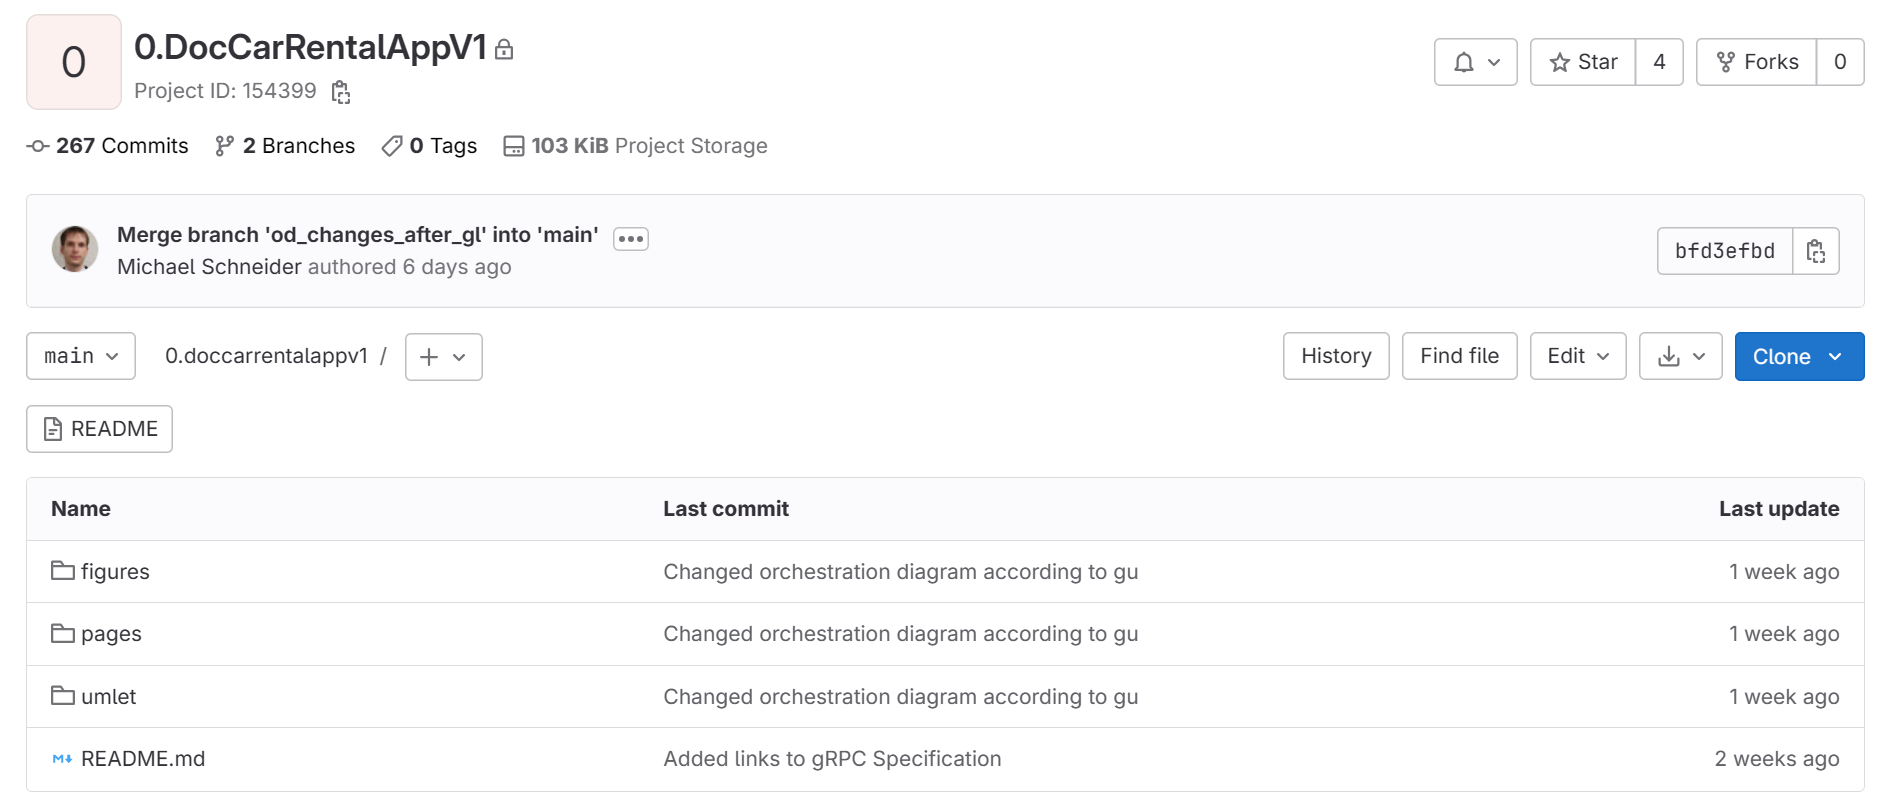
\includegraphics[width=\textwidth]{figures/microservices/introduction/ms_intro_docRepo.png}
    \caption{Documentation Repository of the Car Rental App V1.0}
    \label{fig:doc_repo_car_rental_app_v1}
\end{figure}

\subsubsection*{Type of Architecture and Diagram}
As mentioned above, the diagrams can be found exported as images in the figures folder and as UMLet files in the UMLet folder.
Therefore the architecture diagram can be found in \texttt{0.doccarrentalappv1/figures/ad\_dm-car\_v1.0.png} and \hfill \linebreak \texttt{0.doccarrentalappv1/umlet/cd\_car\_rental\_app\_v1.0.uxf} respectively.
It is a component diagram, showing the components representing the different layers of the architecture and their dependencies.
They can be separated into the presentation layer (UI), the application logic layer (application microservice), the domain logic layer (domain microservice), and the infrastructure layer (databases).

\subsubsection*{Extension of the Architecture}
\texttt{CarRentalAppV1.0}'s deployment diagram is shown in \autoref{fig:system_plus_software_car_rental_app_v1}.
Each component is deployed as a separate and independent microservice.
The deployment is defined by a dedicated Docker file.
These files specify dependencies and the overall environment for each component.
Therefore, each component can be containerized and deployed seamlessly within the same Kubernetes cluster.
Each cluster can be hosted on any chosen cloud provider.
This gives a certain flexibility in terms of deployment options.


\begin{figure}
    \centering
    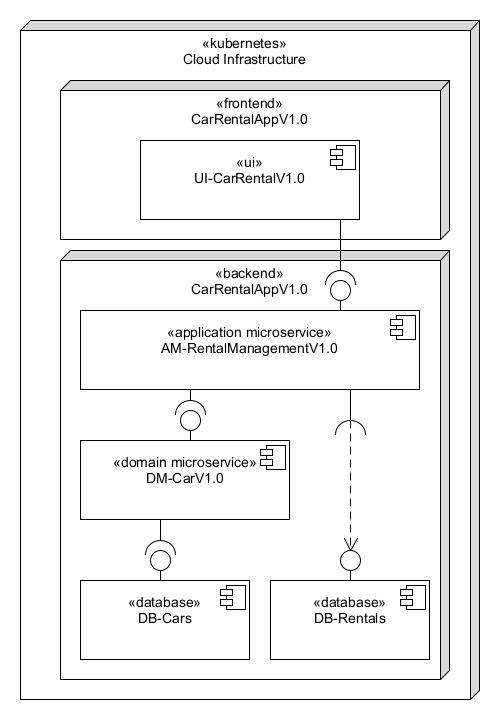
\includegraphics[width=0.5\textwidth]{figures/microservices/introduction/ms_dmCar_SPScarRental.png}
    \caption{SystemPlusSoftware Diagram of the Car Rental App V1.0}
    \label{fig:system_plus_software_car_rental_app_v1}
\end{figure}
